% chapter3.tex -- de (German)
\chapter{Installation der Software}
Eigentlich ist die Installation der Software \textit{babyleicht} und man
muss (Achtung: Unwort!) \textit{nur} den \cmd{one-line-installer} von
\textit{MiczFlor} auf einem jungfr�ulichen \os{Raspbian} starten\dots\\
\url{https://github.com/MiczFlor/RPi-Jukebox-RFID#installation}

\textbf{Aber:}\\
Aufgrund vieler Anfragen der mittlerweile relativ gro�en Community rund
um die {\Bezeichnung} und der daraus resultierenden zahlreichen
\textit{Push Requests} auf github und auch wegen vieler anderer guter
Gr�nde schleichen sich in die an sich gro�artige Arbeit von
\textit{MiczFlor} naturbedingt immer wieder kleinere Fehler ein, die
insbesondere f�r unbedarfte Neulinge bisweilen schwer zu finden und zu
beseitigen sind.

\section{\os{Raspbian Buster Lite} auf dem {\RPi} installieren}
Einige Tutorials im Internet empfehlen zwar, die Software f�r die
{\Bezeichnung} unter \os{Raspbian Buster with desktop} zu installieren,
aber da es sich bei der {\Bezeichnung} um ein einfaches
stand\-alone-System ohne Bildschirm handelt, ist es in meinen Augen
v�llig ausreichend, die Installation auf dem wesentlich kleineren
\os{Raspbian lite} vorzunehmen. Ein X11-Desktop ist schlichtweg nicht
erforderlich. Au�erdem reicht f�r \os{Raspbian Buster Lite} eine
SD-Karte mit einer Speicherkapazit�t von 4GB.

\subsection{Erstellen einer SD-Karte f�r den {\RPi} mit \os{Raspbian Buster Lite}}
Zun�chst wird die aktuelle Version von \os{Raspbian Buster Lite} von der
Homepage der {\foundation}
(\url{https://www.raspberrypi.org/downloads/raspbian/}, ca. 450MiB)
heruntergeladen und entpackt (1,8GiB). Das entpackte Image wird mit
einem daf�r vorgesehenen Programm wie \software{win32diskimager} oder
am Linux-PC mit dem systemeigenen Kommando \cmd{dd} auf die SD-Karte
\textit{geflasht}, um das Image 1:1 zu �bertragen.
\begin{bclogo}[arrondi = 0.2, logo = \bcinfo, ombre = true, epOmbre = 0.25, couleurOmbre = black!30,blur]{Achtung}
Es reicht nicht, die Imagedatei einfach auf eine bereits formatierte
SD-Karte zu kopieren!
\end{bclogo}
% \textbf{Es reicht
%nicht, die Imagedatei einfach auf eine bereits formatierte SD-Karte zu
%kopieren!}\\
Die Details des \textit{Flashens} von Betriebssystem-Images auf eine
SD-Karte werden von der {\foundation} unter
\url{https://www.raspberrypi.org/documentation/installation/installing-images/README.md}
ausf�hrlich beschrieben und in diesem Dokument als bekannt
vorausgesetzt.

Nach dem Flashen enth�lt die SD-Karte zwei Partitionen:
\begin{compactitem}
\item{die FAT32-formatierte \filenam{/boot}-Partition}
\item{die ext4-formatierte Rootpartition von \os{Raspbian}}
\end{compactitem}
\begin{bclogo}[logo = \bclampe, noborder = true]{Hinweis}
Beim (erneuten) Anstecken der SD-Karte am PC werden diese beiden
Partitionen im Dateimanager angezeigt. Sollte auf dem PC jedoch das
Betriebssystem \os{Windows} verwendet werden, so wird nur die
FAT32-formatierte \filenam{/boot}-Partition erkannt.
\end{bclogo}

\subsection{Anmeldung am {\RPi} �ber \software{ssh}}
\begin{figure}[h]
\centering
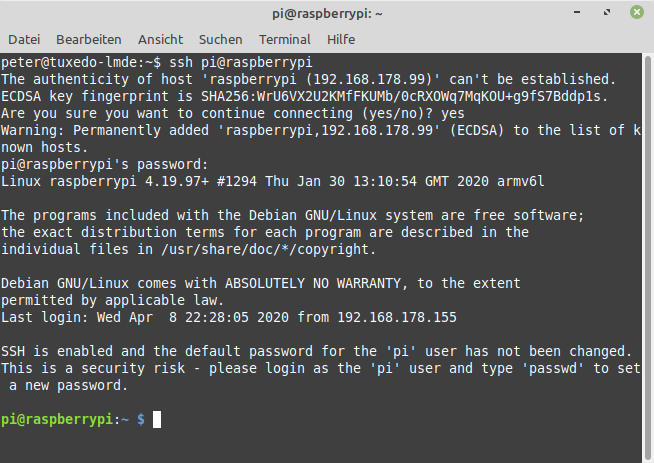
\includegraphics[width=0.80\textwidth, angle=0]{software/login.png}
\caption{erster Login �ber \software{ssh}}
\label{fig:ssh_login}
\end{figure}
Da an den {\RPi} f�r die {\Bezeichnung} weder Bildschirm noch Tastatur
angeschlossen werden, muss der Zugriff auf den {\RPi} von Anfang an �ber
\software{ssh} erfolgen. Dazu muss auf der Partition \filenam{/boot} der
SD-Karte die leere Datei \filenam{ssh} angelegt werden.\\
Nun wird die SD-Karte in den {\RPi} gesteckt, der {\RPi} am besten �ber
Ethernet ans LAN geh�ngt und eingeschaltet. Nach sp�testens einer Minute
sollte \os{Raspbian Buster Lite} vollst�ndig gebootet und der {\RPi} im
LAN bekannt sein. Auf dem PC wird in einem Terminalfenster
(unter \os{Windows} in der Eingabeaufforderung \cmd{cmd.exe}) die
Software \software{ssh} mit folgendem Kommando gestartet:

\cmdPC{ssh pi@raspberrypi}\comment{Das Passwort lautet \texttt{raspberry}}

Die Bildschirmausgabe sieht in etwa wie in Abbildung \ref{fig:ssh_login}
aus.

\subsection{\os{Raspbian} konfigurieren}
Nach erfolgreichem \software{ssh}-Login muss das System jetzt auf einen
aktuellen und sicheren Stand gebracht werden:\\
\cmdPi{sudo apt update \&\& sudo apt upgrade}\comment{System auf den neuesten Stand bringen}\\
\cmdPi{sudo raspi-config}\\
\stdout{1 Change User Password \ \ \ \ \ \ \ \ \ \ \ \ \ \ \ \ \ \ \ \ \ \ \ \ \ \ \ }\comment{Passwort unbedingt �ndern!}\\
\stdout{2 Network Options \ \ \ \ \ --> N1 Hostname \ \ \ \ \ \ \ \ \ \ \ \ }\comment{\zB \texttt{phoniebox1}}\\
\stdout{3 Boot Options \ \ \ \ \ \ \ \ --> B1 Desktop / CLI \ \ \ \ \ \ \ \ --> B2 Console Autologin}\\
%\stdout{4 Localisation Options --> I1 Change Locale \ \ \ \ \ \ \ }\comment{Landeseinstellungen}\\
\stdout{4 Localisation Options --> I2 Change Timezone \ \ \ \ \ }\comment{Zeitzone anpassen}\\
\stdout{\textcolor{white}{ \ \ \ \ \ \ \ \ \ \ \ \ \ \ \ \ \ \ \ \ \ \ } --> I4 Change Wi-fi Country }\comment{diese Anpassung ist ganz wichtig!}\\
\stdout{5 Interfacing Options \ --> P2 SSH}

\subsection{WLAN einrichten}
Da die {\Bezeichnung} ein tragbares Ger�t f�r's Kinderzimmer werden
soll, muss eine WLAN-Ver\-bin\-dung eingerichtet werden:\\
\cmdPi{sudo nano /boot/wpa-supplicant.conf}\\
\editor{country=DE\\
        ctrl\_interface=DIR=/var/run/wpa\_supplicant GROUP=netdev\\
        update\_config=1\\
        \\
        network=\{\\
        \textcolor{white}{\ \ \ \ }ssid="linksys"\\
        \textcolor{white}{\ \ \ \ }psk="{<network-password>}"\\
        \textcolor{white}{\ \ \ \ }key\_mgmt=WPA-PSK\\
        \}
       }

\cmdPi{sudo systemctl restart dhcpcd}\\
\stdout{Warning: The unit file, source configuration file or drop-ins of dhcpcd.service changed on disk. Run 'systemctl daemon-reload' to reload units.}\\
\cmdPi{sudo systemctl daemon-reload}\\
\cmdPi{sudo reboot}\comment{Braucht's das?}\\
\cmdPi{ip addr}\\
\stdout{1: lo: <LOOPBACK\,UP\,LOWER\_UP> mtu 65536 qdisc noqueue state UNKNOWN group default qlen 1000\\
        \textcolor{white}{\ \ \ \ }link/loopback 00:00:00:00:00:00 brd 00:00:00:00:00:00\\
        \textcolor{white}{\ \ \ \ }inet 127.0.0.1/8 scope host lo\\
        \textcolor{white}{\ \ \ \ \ \ \ }valid\_lft forever preferred\_lft forever\\
        \textcolor{white}{\ \ \ \ }inet6 ::1/128 scope host\\
        \textcolor{white}{\ \ \ \ \ \ \ }valid\_lft forever preferred\_lft forever\\
        2: eth0: BROADCAST\,MULTICAST\,UP\,LOWER\_UP> mtu 1500 qdisc pfifo\_fast state UP group default qlen 1000
        \textcolor{white}{\ \ \ \ }link/ether b8:27:eb:70:91:db brd ff:ff:ff:ff:ff:ff\\
        \textcolor{white}{\ \ \ \ }inet 192.168.178.99/24 brd 192.168.178.255 scope global dynamic noprefixroute eth0\\
        \textcolor{white}{\ \ \ \ \ \ \ }valid\_lft 859570sec preferred\_lft 751570sec\\
        \textcolor{white}{\ \ \ \ }inet6 fe80::99ec:954c:4542:ed0/64 scope link \\
        \textcolor{white}{\ \ \ \ \ \ \ }valid\_lft forever preferred\_lft forever\\
        3: wlan0: <BROADCAST\,MULTICAST\,UP\,LOWER\_UP> mtu 1500 qdisc pfifo\_fast state UP group default qlen 1000\\
        \textcolor{white}{\ \ \ \ }link/ether b8:27:eb:63:3a:f2 brd ff:ff:ff:ff:ff:ff\\
        \textcolor{white}{\ \ \ \ }inet 192.168.178.154/24 brd 192.168.178.255 scope global dynamic noprefixroute wlan0\\
        \textcolor{white}{\ \ \ \ \ \ \ }valid\_lft 863877sec preferred\_lft 755877sec\\
        \textcolor{white}{\ \ \ \ }inet6 fe80::3d3b:d9af:5ca6:e45e/64 scope link\\
        \textcolor{white}{\ \ \ \ \ \ \ }valid\_lft forever preferred\_lft forever
       }
%\begin{bclogo}[arrondi = 0.2, logo = \bcinfo, ombre = true, epOmbre = 0.25, couleurOmbre = black!30,blur]{Achtung}
\begin{bclogo}[logo = \bclampe, noborder = true]{Hinweis}
Es wird \textbf{keine} statische IP-Adresse eingerichtet!
\end{bclogo}


\section{Installation der \Bezeichnung-Software}
bla bla





\section{Software / Installation}
ReadMe einbinden...

\subsection{offen}
Reduzierung der Bootzeit\\
automatisch aus nach 15 min.
